\documentclass{article}

\usepackage{tikz}
\usetikzlibrary{arrows,automata,positioning}
\usetikzlibrary{shapes.geometric}
\usepackage{helvet}
\tikzset{every picture/.style={/utils/exec={\sffamily\scriptsize}}}

\usepackage{hyperref}

\begin{document}

\title{Lorem ipsum}

\maketitle

\begin{abstract}
  Lorem ipsum dolor sit amet, consectetur adipiscing elit, sed do eiusmod tempor incididunt ut labore et dolore magna aliqua. Ut enim ad minim veniam, quis nostrud exercitation ullamco laboris nisi ut aliquip ex ea commodo consequat. Duis aute irure dolor in reprehenderit in voluptate velit esse cillum dolore eu fugiat nulla pariatur. Excepteur sint occaecat cupidatat non proident, sunt in culpa qui officia deserunt mollit anim id est laborum.
\end{abstract}

%%%%%%%%%%%%%%

\section{TikZ Example}

See \url{https://www.overleaf.com/learn/latex/LaTeX_Graphics_using_TikZ%3A_A_Tutorial_for_Beginners_(Part_1)%E2%80%94Basic_Drawing} for a TikZ tutorial.

Lorem ipsum dolor sit amet, consectetur adipiscing elit, sed do eiusmod tempor incididunt ut labore et dolore magna aliqua. Ut enim ad minim veniam, quis nostrud exercitation ullamco laboris nisi ut aliquip ex ea commodo consequat. Duis aute irure dolor in reprehenderit in voluptate velit esse cillum dolore eu fugiat nulla pariatur. Excepteur sint occaecat cupidatat non proident, sunt in culpa qui officia deserunt mollit anim id est laborum.

\begin{figure}[htb]
  \centering
  \scalebox{0.5}{
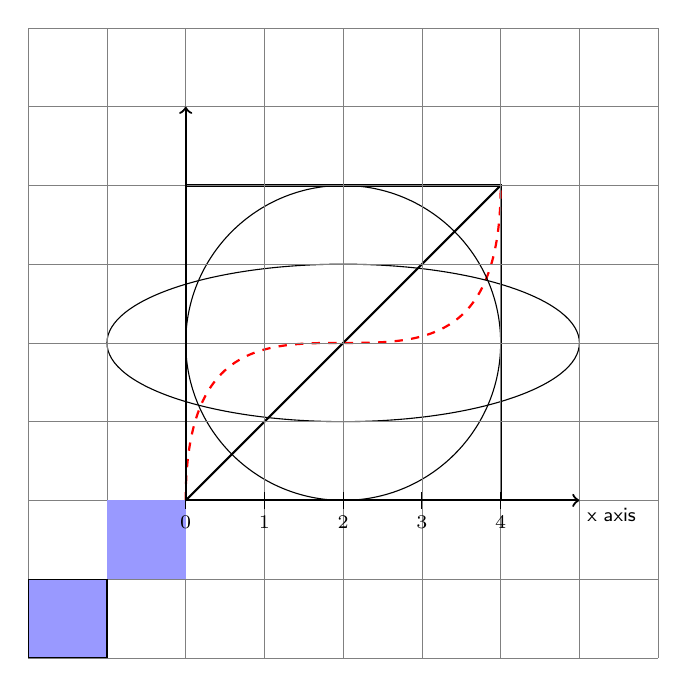
\begin{tikzpicture}
  \draw[thick] (0,0) -- (4,4);
  
  \draw[thick] (0,0) -- (4,0) -- (4,4) -- (0,4) -- cycle;

  \draw[red,thick,dashed] (0,0) .. controls (0,4) and (4,0) .. (4,4);

  \draw (2,2) circle (2);

  \draw (2,2) ellipse (3 and 1);

  \draw[step=1,gray,very thin] (-2,-2) grid (6,6);

  \fill[blue!40!white] (-1,-1) rectangle (0,0);

  \filldraw[fill=blue!40!white, draw=black] (-2,-2) rectangle (-1,-1);

  \draw[thick,->] (0,0) -- (5,0) node[anchor=north west] {x axis};
  \foreach \x in {0,1,2,3,4}
  \draw (\x,3pt) -- (\x,-3pt) node[anchor=north] {$\x$};

  \draw[thick,->] (0,0) -- (0,5);
\end{tikzpicture}
}
\caption{TikZ Example}
\end{figure}

%%%%%%%%%%%%%%

\section{Activity-centric Example}

Lorem ipsum dolor sit amet, consectetur adipiscing elit, sed do eiusmod tempor incididunt ut labore et dolore magna aliqua. Ut enim ad minim veniam, quis nostrud exercitation ullamco laboris nisi ut aliquip ex ea commodo consequat. Duis aute irure dolor in reprehenderit in voluptate velit esse cillum dolore eu fugiat nulla pariatur. Excepteur sint occaecat cupidatat non proident, sunt in culpa qui officia deserunt mollit anim id est laborum.

\begin{figure}[htb]
  \centering
% nodes spaced 2cm from their centres
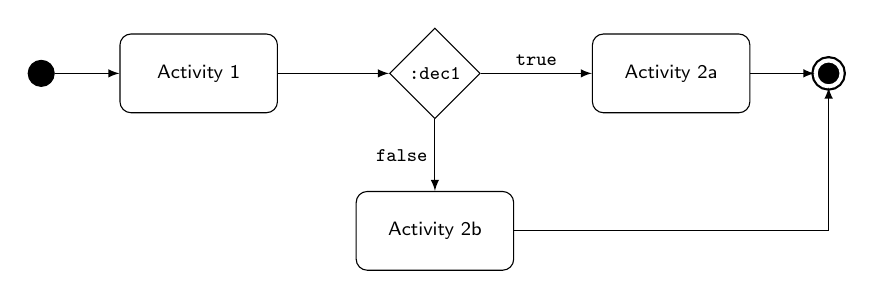
\begin{tikzpicture}[node distance=2cm]
  \tikzstyle{start} = [circle, minimum size=.33cm, draw=black, fill=black]
  \tikzstyle{end} = [circle, minimum size=.33cm, draw=black, fill=black, double=white, double distance=1.5pt, thick]
  \tikzstyle{activity} = [rectangle, rounded corners, minimum height=1cm, minimum width=2cm, text centered, draw=black]
  \tikzstyle{decision} = [diamond, text centered, draw=black]

  \tikzstyle{arrow} = [-latex] %,>=stealth]

  \node (start) [start] {};
  \node (act1) [activity, right of=start] {Activity 1};
  \node (dec1) [decision, right of=act1, xshift=1cm] {\tt :dec1};
  \node (act2a) [activity, right of=dec1, xshift=1cm] {Activity 2a};
  \node (act2b) [activity, below of=dec1] {Activity 2b};
  \node (end) [end, right of=act2a] {};

  \draw [arrow] (start) -- (act1);
  \draw [arrow] (act1) -- (dec1);
  \draw [arrow] (dec1) -- node[anchor=south] {\tt true} (act2a);
  \draw [arrow] (dec1) -- node[anchor=east] {\tt false} (act2b);
  % vertical then horizontal
  \draw [arrow] (act2b) -| (end);
  \draw [arrow] (act2a) -- (end);
\end{tikzpicture}
\caption{UML-style activity-centric process example (with textual descriptions for nodes and edges, identifier for decision)}
\end{figure}

%%%%%%%%%%%%%%

\section{State-centric Example}

Lorem ipsum dolor sit amet, consectetur adipiscing elit, sed do eiusmod tempor incididunt ut labore et dolore magna aliqua. Ut enim ad minim veniam, quis nostrud exercitation ullamco laboris nisi ut aliquip ex ea commodo consequat. Duis aute irure dolor in reprehenderit in voluptate velit esse cillum dolore eu fugiat nulla pariatur. Excepteur sint occaecat cupidatat non proident, sunt in culpa qui officia deserunt mollit anim id est laborum.

\subsection{UML Style}

Lorem ipsum dolor sit amet, consectetur adipiscing elit, sed do eiusmod tempor incididunt ut labore et dolore magna aliqua. Ut enim ad minim veniam, quis nostrud exercitation ullamco laboris nisi ut aliquip ex ea commodo consequat. Duis aute irure dolor in reprehenderit in voluptate velit esse cillum dolore eu fugiat nulla pariatur. Excepteur sint occaecat cupidatat non proident, sunt in culpa qui officia deserunt mollit anim id est laborum.


\begin{figure} [htb]
  \centering
% nodes spaced 2cm from their centres
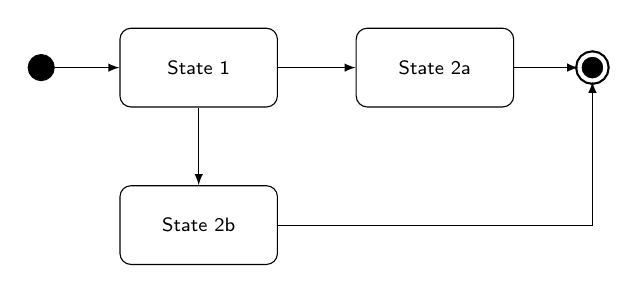
\begin{tikzpicture}[node distance=2cm]
  \tikzstyle{start} = [circle, minimum size=.33cm, draw=black, fill=black]
  \tikzstyle{end} = [circle, minimum size=.33cm, draw=black, fill=black, double=white, double distance=1.5pt, thick]
  \tikzstyle{state} = [rectangle, rounded corners, minimum height=1cm, minimum width=2cm, text centered, draw=black]

  \tikzstyle{arrow} = [-latex] %,>=stealth]

  \node (start) [start] {};
  \node (state1) [state, right of=start] {State 1};
  \node (state2a) [state, right of=state1, xshift=1cm] {State 2a};
  \node (state2b) [state, below of=state1] {State 2b};
  \node (end) [end, right of=state2a] {};

  \draw [arrow] (start) -- (state1);
  \draw [arrow] (state1) -- (state2a);
  \draw [arrow] (state1) -- (state2b);
  % vertical then horizontal
  \draw [arrow] (state2a) -- (end);
  \draw [arrow] (state2b) -| (end);
\end{tikzpicture}
\caption{UML-style state-centric process example (with textual descriptions for nodes and edges)}
\end{figure}

\subsection{Formal Methods Style}

Lorem ipsum dolor sit amet, consectetur adipiscing elit, sed do eiusmod tempor incididunt ut labore et dolore magna aliqua. Ut enim ad minim veniam, quis nostrud exercitation ullamco laboris nisi ut aliquip ex ea commodo consequat. Duis aute irure dolor in reprehenderit in voluptate velit esse cillum dolore eu fugiat nulla pariatur. Excepteur sint occaecat cupidatat non proident, sunt in culpa qui officia deserunt mollit anim id est laborum.

\begin{figure} [htb]
  \centering
% nodes spaced 2cm from their centres
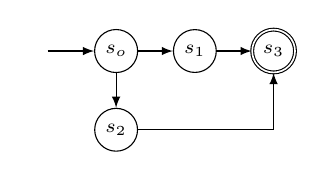
\begin{tikzpicture}[node distance=1cm]
  \tikzstyle{start} = [circle, draw=none, fill=none]
  \tikzstyle{state} = [circle, text centered, draw=black]
  
  \tikzstyle{arrow} = [-latex] %,>=stealth]

  \node (start) [start] {};
  \node (state1) [state, right of=start] {$s_o$};
  \node (state2a) [state, right of=state1] {$s_1$};
  \node (state2b) [state, below of=state1] {$s_2$};
  \node (state3) [state, double, right of=state2a] {$s_3$};

  \draw [arrow] (start) -- (state1);
  \draw [arrow] (state1) -- (state2a);
  \draw [arrow] (state1) -- (state2b);
  % vertical then horizontal
  \draw [arrow] (state2a) -- (state3);
  \draw [arrow] (state2b) -| (state3);
\end{tikzpicture}
\caption{Formal-methods-style state-centric process example (with identifiers for states and transitions)}
\end{figure}


\end{document}
